\begin{homeworkProblem}
  Sean $E$ y $F$ espacios vectoriales normados. Suponga que $E$ es de dimensión finita ($F$ no necesariamente de dimensión finita).
  \begin{enumerate}[(i)]
    \item Muestre que todas las normas asignadas a $E$ son equivalentes\footnote{Sean $\norm{\cdot}_{1}$ y $\norm{\cdot}_{2}$ dos normas sobre $E$. Recordemos que dos normas son equivalentes si existen constantes positivas $c_1$ y $c_2$, tales que $c_1\norm{x}_{1}\leq \norm{x}_{2}\leq c_2\norm{x}_{1}$, para todo $x\in E$.}.
    \item Muestre que toda transformación lineal $T:E\to F$ es continua.
    \item De un ejemplo donde se verifique que (II) puede ser falsa si $E$ es de dimensión infinita. 
  \end{enumerate}
  \begin{solution}
    \begin{enumerate}[(i)]
      \item Suponga $\norm{\cdot}_{1}$ y $\norm{\cdot}_{2}$ normas de $E$ espacio vectorial de dimensión finita.\\
        En particular, como $E$ es de dimensión finita sabemos que existe una base\\
        $\mathcal{B}=\{e_1,e_2,\cdots,e_n\}\subset E$ tal que si tomamos $x\in E$, entonces
        \begin{align*}
          x=\sum_{i=1}^{n}x_ie_i, &&\text{con $x_i$ escalares de $E$.}
        \end{align*}
        Ahora, fijemos $\norm{x}_1$ como 
        \begin{align*}
          \norm{x}_{1}=\sum_{i=1}^{n}|x_i|
        \end{align*}
        Además, note que en general para $\norm{x}_2$ se tiene que
        \begin{align*}
          \norm{x}_{2}&=\norm{\sum_{i=1}^{n}x_ie_i}_{2},\\
          &\leq \sum_{i=1}^{n}\norm{x_ie_{i}}_{2},\\
          &\leq \sum_{i=1}^{n}|x_i|\norm{e_i}_{2},\\
          &\leq \max_{i=1,\cdot,n}\norm{e_i}_{2}\sum_{i=1}^{n}|x_i|,\\
          &\leq c_{2}\norm{x}_{1}.
        \end{align*}
        Por otro lado, queremos ver que existe $c_1>0$ tal que $c_1\norm{x}_{1}\leq \norm{x}_{2}$ para todo $x\in E$, en particular, note que si definimos $A=\{x\in E: \norm{x}_{1}=1\}$, nos queda que esperamos que se cumpla $c_1\leq \norm{x}_{2}$ para todo $x\in A$.\\
        Note que como $A$ es cerrado y acotado (en $\norm{\cdot}_{1}$) y $E$ es de dimensión finita, entonces $A$ es compacto, además, veamos que $\norm{x}_{2}$ es continua en la topología de $\norm{\cdot}_{1}$.
        Note que dado $\epsilon>0$ existe $\delta=\frac{\epsilon}{c_2}>0$ tal que si
        \begin{align*}
          \norm{x-y}_{1}<\delta
        \end{align*}
        entonces
        \begin{align*}
          \left| \norm{x}_{2}-\norm{y}_{2} \right|&<\left| \norm{x-y}_{2} \right|,\\
          &<c_2\norm{x-y}_{1},\\
          &<c_2\frac{\epsilon}{c_2},\\
          &<\epsilon.
        \end{align*}
        Luego, como $\norm{\cdot}_{2}$ es continua en $\norm{\cdot}_{1}$, como $A$ es compacto, entonces $\norm{x}_{2}$ alcanza su mínimo en $A$, es decir, existe $z\in A$ tal que $\norm{z}_{2}\leq \norm{x}_{2}$ para todo $x\in A$, luego podemos definir $c_1=\norm{z}_{2}$, por lo que podemos concluir que existen constantes $c_1,c_2>0$ tales que
        \begin{align*}
          c_1\norm{x}_1\leq \norm{x}_{2}\leq c_2\norm{x}_{1} &&\text{para todo $x\in E$.}
        \end{align*}
        Ahora, note que esto nos permite concluir que dadas $2$ normas cualesquiera estas con equivalentes, ya que mediante $\norm{x}_1$ se puede realizar el siguiente cálculo.\\
        Suponga $c_{21}$ y $c_{22}$ las constantes respectivas a la equivalencia entre una norma $\norm{x}_{1}$ y la norma $\norm{x}_{2}$ y por otro lado suponga $c_{31}$ y $c_{32}$ las constantes respectivas a la equivalencia entre la norma $\norm{x}_{1}$ y la norma $\norm{x}_{3}$, veamos que podemos concluir que $\norm{x}_{2}$ y $\norm{x}_{3}$ son equivalentes 
        \begin{align*}
          \norm{x}_{2}\leq c_{22}\norm{x}_1\leq \frac{c_{22}}{c_{31}}\norm{x}_{3},
        \end{align*}
        por otro lado
        \begin{align*}
          \norm{x}_{3}\leq c_{32}\norm{x}_{1}\leq \frac{c_{32}}{c_{21}}\norm{x}_{2},
        \end{align*}
        de lo que se puede concluir que
        \begin{align*}
          \frac{c_{31}}{c_{22}}\norm{x}_{2}\leq\norm{x}_{3}\leq \frac{c_{32}}{c_{21}}\norm{x}_{2},
        \end{align*}
        es decir, las normas $\norm{\cdot}_{2}$ y $\norm{\cdot}_{3}$ son equivalentes, luego como estas son arbitrarias se puede concluir que todas las normas asignadas a $E$ son equivalentes.
      \item Suponga $T:E\to F$ transformación lineal.\\
        Note que como $E$ es de dimensión finita, podemos asumir que existe una base\\
        $\mathcal{B}:=\{e_1,e_2,\cdots,e_n\}$, luego dado $x\in E$ lo podemos expresar de la forma
        \begin{align*}
          x=\sum_{i=1}^{n}x_ie_i.
        \end{align*}
        Ahora, note que como $T$ es una transformación lineal entonces se cumple que
        \begin{align*}
          \norm{Tx}_{F}&=\norm{T\left( \sum_{i=1}^{n}x_ie_i \right)}_{F},\\
          &\leq\sum_{i=1}^{n}|x_i|\norm{Te_i}_{F},\\
          &\leq\sum_{i=1}^{n}|x_i|\max_{i=1,\cdots,n}\norm{Te_i}_{F},\\
          &\leq \max_{i=1,\cdots,n}\norm{Te_i}_{F} \norm{x}_{E},\\
          &\leq M\norm{x}_{E}.
        \end{align*}
        Si tomamos $M=\max_{i=1,\cdots,n}\norm{Te_i}_{F}$, luego $\norm{Tx}_{F}\leq M\norm{x}_{E}$ y por ende el operador es continuo, luego como se tomó $T$ arbitrario se concluye que toda transformación lineal de $E$ a $F$ con $E$ de dimensión finita es continua.
      \item Suponga $T:(C[0,2],\norm{\cdot}_{1})\to(C[0,2],\norm{\cdot}_{\infty})$ tal que $Tf=f$.\\
      Suponga 
      \begin{align*}
        f_k(x)= 
        \begin{cases}
          0, &\text{ si } x\in\left[0,\frac{2k-1}{2k}\right]\cup\left[\frac{2k+1}{2k},2\right] \text{,} \\
          2k^2x-2k^2+k, &\text{ si } x\in\left[\frac{2k-1}{2k},1\right],\\
          -2k^2x+2k^2+k, &\text{ si } x\in\left[1,\frac{2k+1}{2k}\right].
        \end{cases}
      \end{align*}
      Se puede verificar que $\norm{f_k}_{1}=1$, no obstante note que $f_{k}(1)=k$, por lo que funciona como ejemplo para verificar que
      \begin{align*}
        \sup_{\substack{f_k}}\norm{f_{k}}_{\infty}=\infty.
      \end{align*}
      Luego no existe $M>0$ tal que 
      \begin{align*}
        \norm{f}_{\infty}\leq M\norm{f}_{1}.
      \end{align*}
      Con la intención de ser gráfico con el ejercicio veamos la gráfica para algunos valores de $k$.
      \begin{figure}[H]
      \begin{center}
        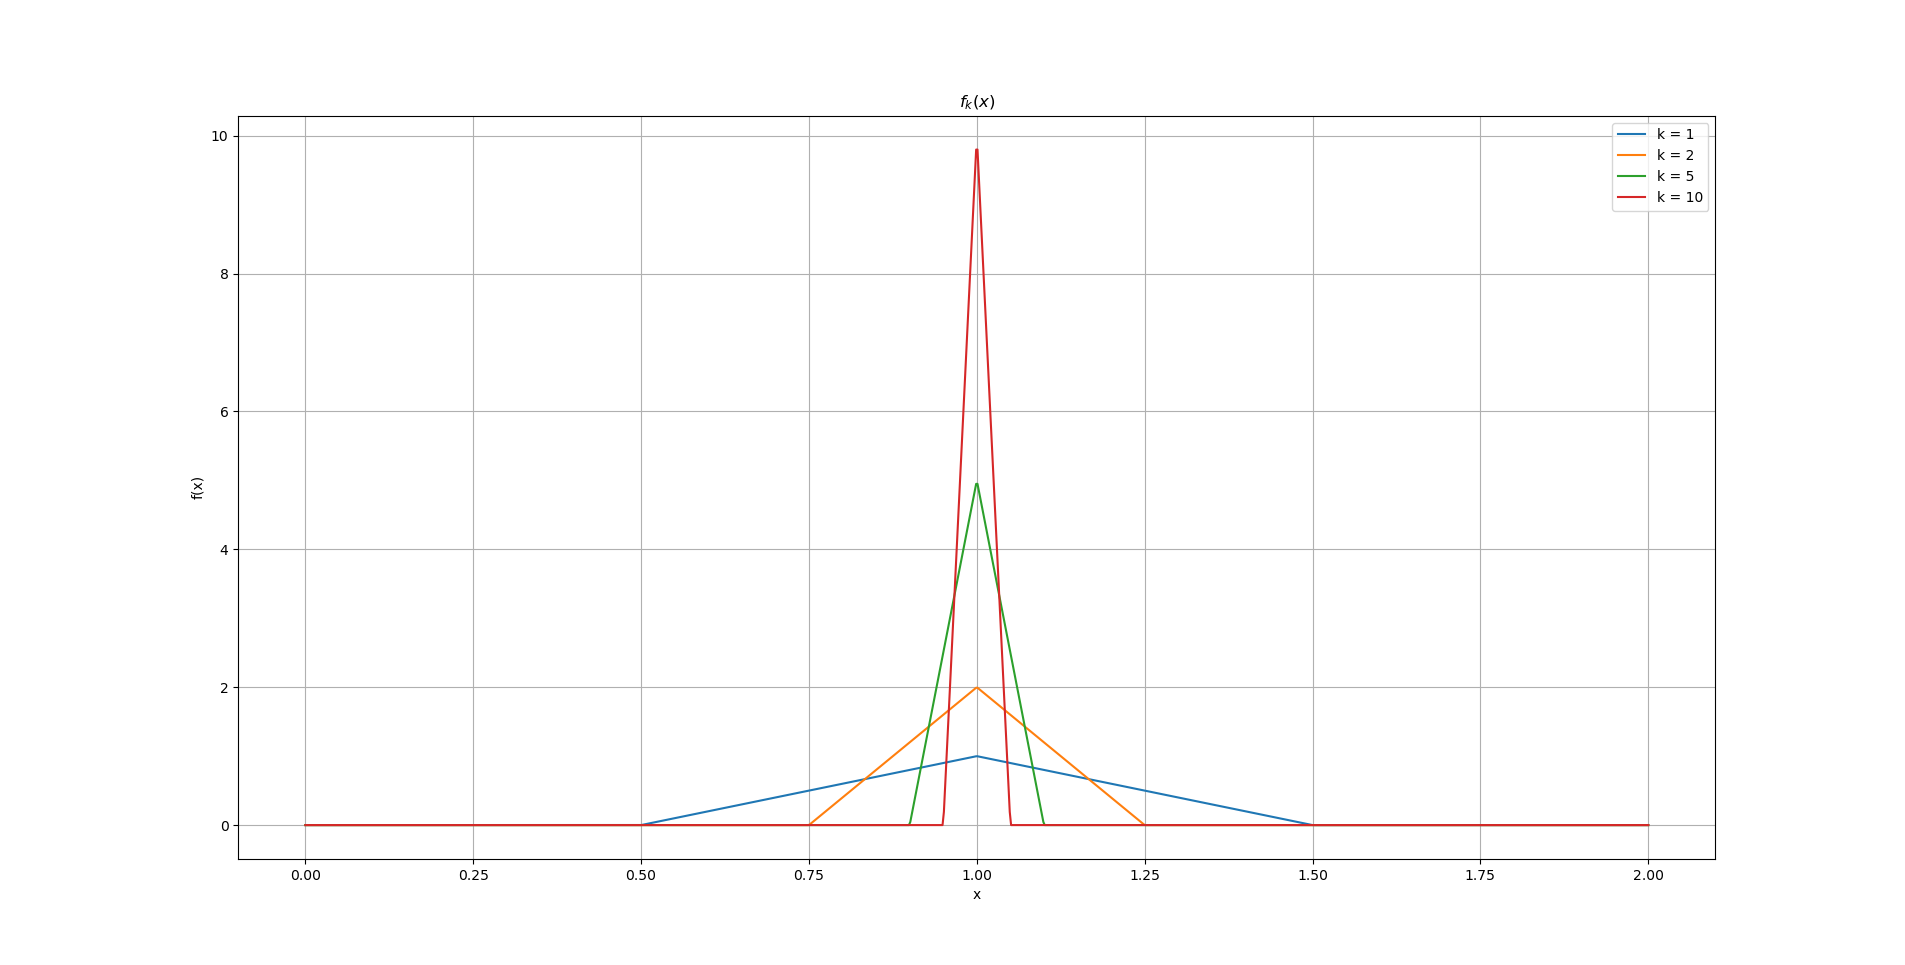
\includegraphics[scale=0.33]{Figures/graficacontraejemplo.png}
      \end{center}
        \caption{$f_k(x)$ con $k=1,2,5$ y $10$.}
      \end{figure} 
    \end{enumerate}
  \end{solution}
\end{homeworkProblem}
